\documentclass[letterpaper, 10pt]{article}

\usepackage[english]{custompack}
\usepackage{fullpage}
%\usepackage{hyperref}
%\usepackage{abcproblem}
\usepackage{listings}
\usepackage{wrapfig}
%\renewcommand{\thesubsection}{\alph{subsection}}

%\allowdisplaybreaks
\numberwithin{theorem}{section}

% (fold)
\lstset{ 
	basicstyle=\ttfamily,%\footnotesize,
	keywordstyle=\color{blue}, 
	commentstyle=\color{gray}, 
	stringstyle=\color{darkgreen}, 
	emphstyle=\color{purple},
	%identifierstyle=, %vanlige ting
	numbers=left, 
	numberstyle=\footnotesize\ttfamily\color{gray}, 
	numbersep=1em,
	stepnumber=1, 
	%firstnumber=last, % dersom listingen deles i to, forsett der man slapp
	firstnumber=1,
	showspaces=false, 
	showstringspaces=false,
	captionpos=b,
	%frame=single,
	breakatwhitespace,
	breaklines=true, 
	tabsize=4,
	% python-spesifikt: 
	language=python,
	morekeywords={None, True, False, with, as, yield, self}, 
	emph={tuple, int, append, raw_input, upper, map, reduce, filter, len, str, open, hex, bin, format, range, xrange, title, strip, split, pop, join, min, max, sum, chr, set, list, sort, sorted, reversed, enumerate, ValueError, TypeError, IndexError, dict, zip, ord, any, all, count, Exception, __init__, __str__, __repr__, __class__, __name__, KeyboardInterrupt, hash, items, add, lower, upper, float}
}
% (end)

\title{\textbf{Assignment 1}}
\author{Håkon Mork \\ ESCE 526 Artificial Intelligence}
\date{\today}

\begin{document}
\maketitle
\noindent

\section{}
\subsection{Number of states visited with simple heuristic}
Game A:
\begin{table}[h]
	\centering
	\small
	\begin{tabular}{lrrrr}
		Cutoff depth & 3 & 4 & 5 & 6 \\
		\midrule
		Minmax & 77,445 & 1,276,689 & 21,335,620 &  Unknown \\
		$\alpha$-$\beta$ pruning & 4129 & 48,203 & 694,652 & Unknown \\
		\midrule
		Improvement & $\times$18.76 & $\times$26.49 & $\times$30.72 & Unknown
	\end{tabular}
\end{table}

\noindent Game B:
\begin{table}[h]
	\centering
	\small
	\begin{tabular}{lrrrr}
		Cutoff depth & 3 & 4 & 5 & 6 \\
		\midrule
		Minmax & 98,345 & 1,704,319 & 29,770,996 & Unknown \\
		$\alpha$-$\beta$ pruning & 6421 & 96,884 & 1,683,194 & Unknown \\
		\midrule
		Improvement & $\times$15.32 & $\times$17.59 & $\times$17.69 & Unknown
	\end{tabular}
\end{table}

\noindent Game C:
\begin{table}[h]
	\centering
	\small
	\begin{tabular}{lrrrr}
		Cutoff depth & 3 & 4 & 5 & 6 \\
		\midrule
		Minmax & 69,954 & 1,237,535 & 22,191,032 & Unknown \\
		$\alpha$-$\beta$ pruning & 3763 & 51,098 & 840,633 & Unknown \\
		\midrule
		Improvement & $\times$18.59 & $\times$24.22 & $\times$26.40 & Unknown
	\end{tabular}
\end{table}

\noindent This game has a high branching factor, in the ballpark of about 16 possible moves for each round, which makes exploring the game tree to any significant depth a very time-consuming chore. I didn't have time to calculate the numbers for cutoff depth 6, but they should be at least one order of magnitude higher than for the previous depth. Depressingly, I also found a bug in my program shortly before the submission deadline, so I'm worried that I have miscalculated the minmax figures. An interesting observation is that alpha-beta pruning seems to be increasingly efficient at chopping off irrelevant branches of the game tree as the cutoff depth increases.\footnote{In my code I consider the children of the current state to be in ply 0; their children, i.e., the grandchildren of the current state, are in ply 1, and so on. If this interpretation is incorrect and the current state's children should instead be regarded as being on ply 1, the values in the tables above should be shifted one column to the right.} Observe, for example, that in game A the number of states visited by minmax with cutoff depth 3 was 18 times higher than the number visited by alpha-beta, while it was over 30 times higher when the cutoff depth was 5.

\subsection{Does state generation order matter?}
My evaluation function iterates through the successor states in the order they were generated: left-to-right, top-to-bottom, with the directions generated in the (arbitrary) order north-east-south-west. I considered the first move in game A and ran\footnote{The commands given were \texttt{python ass1.py --input starta.txt --cutoff 3 --alg ab --count --shuffle}. See the appendix for details on usage.} alpha-beta pruning five times with a cutoff depth of 3, shuffling the list of successor states randomly every time one is generated. (Since the minmax algorithm does not prune the game tree at all, the order in which it evaluates successors is irrelevant.) 

I found that evaluation order \emph{did} matter, though not impressively so. Alpha-beta pruning with the non-shuffled evaluation order visited 4129 states, as per the table above. The sample runs with suffling visited 4480, 4338, 4324, 4114, and 4376 states, respectively, for an average of 4326 states, which is $4.77\%$ more than the non-shuffled case. The maximum deviations from the original order were $8.5\%$ more and $0.36\%$ fewer states visited. (I also tried evaluating states in the reverse order; the difference was negligble.) This suggests that there is no significant benefit to be gained by shuffling; in fact, we see that more states were visited with alternative evaluation orders than with the original sequence. I don't know if this is a coincidence or if the order I picked is somehow optimal; alpha-beta pruning should perform best when the most valuable branches of the game tree are explored early, and most of the subsequent branches are pruned. 

\section{}
\subsection{Choice of evaluation function}
The \texttt{fancyheuristic} function calculates a heuristic value for a given player in a given board state. The heuristic has two parts: one to give a score based on how good the player's position is, and one to give a score for foiling the other player's plans. I underestimated the time it would take to implement a good heuristic, and due to coursework in other subject I didn't get time to work on it as much as I would have liked.

The part of the heuristic that evaluates the value of the board positions is rather simple. Let $n_i$ be the number of $i$-in-a-row instances the player has on the board, either horizontally, vertically, or diagonally. For example, if the player has 3 pieces in a row at two different spots on the board, we have $n_3 = 2$. This number is multiplied by a corresponding power of 10, so that more weight is given to board states with more pieces connected. That is, the score is $\sum_{i=2}^4 n_i \cdot 10^i$. This ensures that the player gets a higher score for having more pieces in a row; that is, having several instances of two pieces connected is by far outweighed by having three pieces connected. Though this is hardly an optimal weighting, from my observations it looks like it performs reasonably well.

\begin{wrapfigure}{l}{0.25\textwidth}
	\centering
	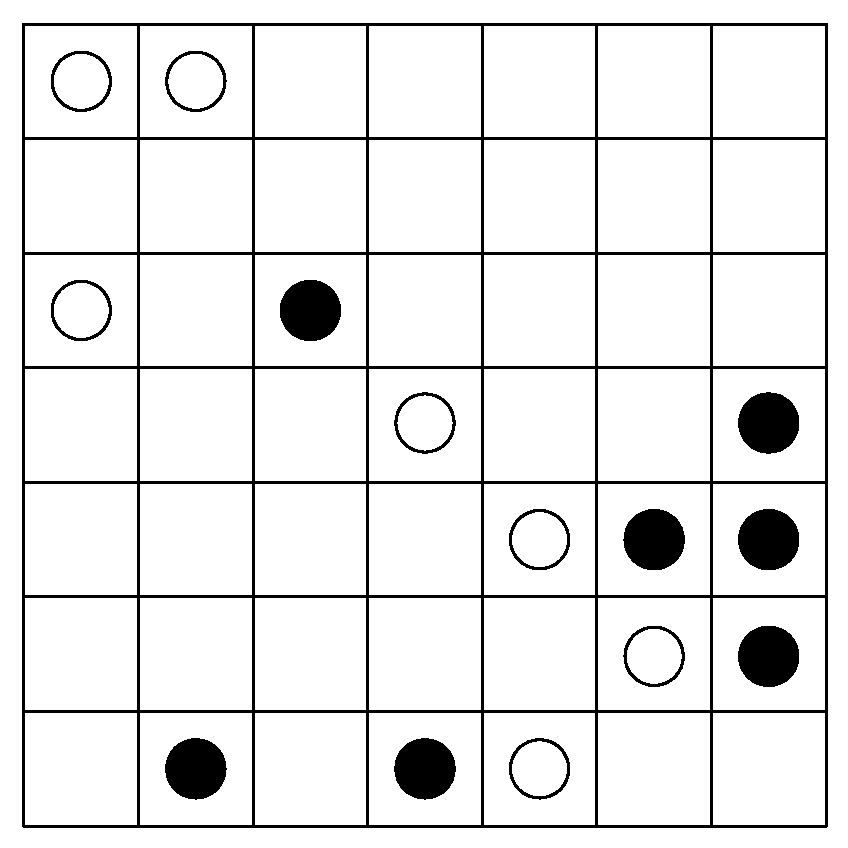
\includegraphics[width=0.24\textwidth]{examplestate}
	\caption{Example position.}
	\label{fig:heuristic}
\end{wrapfigure}
The heuristic also comprises the \texttt{sabotage} function, which gives bonus points for obstructing the opponent. If the opponent has three pieces in a row and is just about to win, placing a piece such that an end of that line is blocked confers a big bonus on that game state's heuristic value. The rationale is that only one thing should be better than hindering the opponent from connecting four pieces: namely, to connect four of one's own pieces. Therefore the penalty or bonus is 9999, which is barely smaller than the 10,000 gained from winning. I haven't been able to say conclusively whether the agent plays better with this addition, but it stands to reason that it should.

As an example of how the heuristic works, consider the situation in figure \ref{fig:heuristic}, where the white player gets $1 \times 10^3 + 2 \times 10^2 = 1200$ points for having that many pieces in a row. The black player gets a bonus for blocking a white connect-4 while collecting $1 \times 10^3 + 1 \times 100 = 1100$ points for the rest of the pieces.

In a sense, my agent follows a greedy algorithm: it follows a (locally) utility-maximizing sequence of actions. Thus, since winning the game has the highest possible heuristic value, the agent will try to achieve that outcome as soon as it can, without any specific regard to the inevitability (or not) of that outcome. Likewise, since losing has low utility but blocking the opponent from winning has high utility, the agent will try to prevent the opponent's victory. It does not specifically try to delay its own defeat, other than in terms of choosing the course of action that maximizes utility. Hopefully those concerns will coincide.

\subsection{Number of states visited with advanced heuristic}
The improved heuristic does \emph{not} consistently reduce the number of states visited, which I found surprising: for example, with alpha-beta pruning and a cutoff depth of 3, it visited 11,152 states, compared to the simple heuristic's 4129 in the first move of game A. With a cutoff depth of 4 it visited 49,254, which is comparable to the simple heuristic's 48,203. With minmax it visits the same number of states since the game tree isn't pruned. While it may be the case that my improved heuristic just isn't any good, it could also be that a significant number of states have the same heuristic value. I find it hard to believe that there should be more of those than all the states with value 0 in the case of the simple heuristic, so I have no plausible explanation.

\subsection{Tradeoff between evaluation function and game tree depth}
The improved heuristic is significantly more computationally intensive, and takes longer to explore the game tree to a given depth than the simple heuristic. An agent using the simple one can thus explore a greater number of states within a given amount of time. While this is certainly a drawback for the advanced heuristic, I found that the agent's gameplay improved significantly, even when severely constrained by time or cutoff depth. In contrast, the simple heuristic, even when given more time and a greater depth, saw my agent explore a vastly greater game tree and still come up with obviously boneheaded decisions. Thus it seems to me that improving the quality of the heuristic is preferable to throwing more hardware at a simple, stupid heuristic to allow it to look even further ahead and explore the state space even more. That is, as long as we can't have our cake and eat it too.

\clearpage
\appendix
\section{Appendix: Source code}
\subsection{Implementation comments}
The implementation is single-threaded, which is obviously not optimal in terms of pure performance. It seems to me that exploring a state space is a problem that lends itself well to parallelization since the subproblems are independent and potentially non-overlapping.

\subsection{Usage}
All arguments are optional:
\begin{itemize}
	\item \texttt{-i} or \texttt{--input}: Specify an input file to be used as the initial game state. A plain-text file following the notation used in the assignment is expected. Defaults to the example illustrated in the ``Introduction'' part of the assignment text.
	\item \texttt{-u} or \texttt{--human}: The computer should play against a human adversary, not just against itself. May take values \texttt{w} or \texttt{b} to indicate that the human should be white or black, respectively. 
	\item \texttt{-c} or \texttt{--cutoff}: Specify a cutoff depth. Defaults to 3.
	\item \texttt{-a} or \texttt{--alg}: Specify which of the minmax or alpha-beta pruning algorithms is to be used. May take values \texttt{mm} or \texttt{ab}. Defaults to alpha-beta pruning.
	\item \texttt{-l} or \texttt{--log}: A log file should be written on exit. May prove useful for the tournament.
	\item \texttt{-k} or \texttt{--count}: Count the number of states visited. Used for problem 1.1.
	\item \texttt{-s} or \texttt{--shuffle}: Shuffle the list of successor states before evaluating them. Used for problem 1.2.
	\item \texttt{-f} or \texttt{--fancy}: Indicate that the advanced heuristic should be used. 
	\item \texttt{-t} or \texttt{--time}: Time limit (in seconds) for each move.
\end{itemize}
Example: \texttt{python ass1.py --input file.txt --alg ab --human w --time 20 --fancy --log}

\subsection{Listing}
The code is written in Python 2.7. I've expunged all logging statements and other debugging aids from this listing for the sake of readability. I find that Python is quite legible in most cases, so I've primarily added comments to explain purpose.
\lstinputlisting{./ass1.py}

\end{document}
